\documentclass[a4paper,11pt]{article}
\usepackage[T1]{fontenc}
\usepackage[utf8]{inputenc}
\usepackage{lmodern}
\usepackage{amsmath}
\usepackage{fullpage} 
\usepackage{graphicx, subfigure}
\usepackage{pgf}
\usepackage{tikz}
\usetikzlibrary{arrows,automata}

\title{Principles of Computer System Design\\Assignment 2}
\author{Robert Schmidtke}

\begin{document}

\maketitle

% -----
% -----
% -----
\section{Exercises}
\label{sec:ex}

% -----
\subsection{Serializability \& Locking}
\label{sec:ex1}

\subsubsection*{(a)}
\begin{figure}[ht]
  \centering
  \subfigure[Precedence graph for Schedule 1]{
    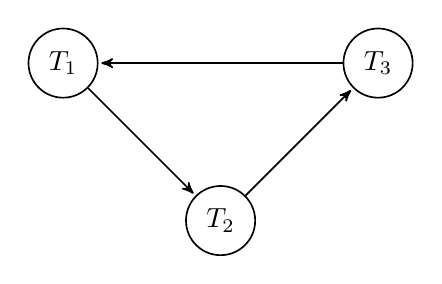
\begin{tikzpicture}[->,>=stealth',shorten >= 1pt,auto,node distance=2.cm,accepting/.style={double distance= 1.5pt},semithick]
      
      \node[state] (T1) {\(T_1\)};
      \node[state] (T2) [below of=T1, right of=T1] {\(T_2\)};
      \node[state] (T3) [above of=T2, right of=T2] {\(T_3\)};    
      
      \path (T1) edge node {} (T2);
      \path (T2) edge node {} (T3); 
      \path (T3) edge node {} (T1);    
      
    \end{tikzpicture}
    \label{fig:prec-schedule1}
  }
  \subfigure[Precedence graph for Schedule 2]{
    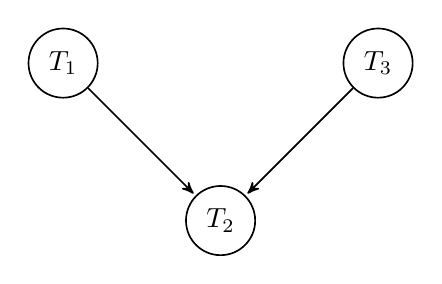
\begin{tikzpicture}[->,>=stealth',shorten >= 1pt,auto,node distance=2.cm,accepting/.style={double distance= 1.5pt},semithick]
      
      \node[state] (T1) {\(T_1\)};
      \node[state] (T2) [below of=T1, right of=T1] {\(T_2\)};
      \node[state] (T3) [above of=T2, right of=T2] {\(T_3\)};
      
      \path (T1) edge node {} (T2);
      \path (T3) edge node {} (T2);
      
    \end{tikzpicture}
    \label{fig:prec-schedule2}
  }
\end{figure}

The precedence graph in figure~\ref{fig:prec-schedule1} for the first schedule contains a cycle which implies that schedule 1 is not conflict-serializable. On the other hand, figure~\ref{fig:prec-schedule2} contains no cycle and thus the schedule is conflict-serializable. A possible serialization of the transactions could be \(T_1 \rightarrow T_3 \rightarrow T_2\).

\subsubsection*{(b)}
Given the cyclic nature of the precedence graph for schedule 1 we can conclude that no strict 2PL scheduler could have generated it. \(T_1\) only releases its shared lock on \(X\) at the very end whereas \(T_2\) acquires the exclusive lock on \(X\) and commits before \(T_1\) meaning that \(T_1\) cannot have had the shared lock on \(X\).

For schedule 2 this is no problem, the only adaption is that \(T_2\) can only read \(Z\) after \(T_3\) has committed since the shared lock is only required after \(T_3\) has released its exclusive lock on \(Z\).
\begin{align*}
  T_1&: &S(X)~&R(X) &     &     &     &  &     &E(Y) &W(Y)~&C &     &     &     &     &\\
  T_2&: &     &     &     &     &S(Z)~&  &R(Z) &     &     &  &E(X)~&W(X) &E(Y)~&W(Y) &C\\
  T_3&: &     &     &E(Z)~&W(Z) &     &C &     &     &     &  &     &     &     &     &
\end{align*}

Where \(S(X)\) means requesting the shared lock and \(E(X)\) means requesting the exclusive lock on \(X\).

% -----
\subsection{Optimistic Concurrency Control}
\label{sec:ex2}
\emph{Scenario 1}: \(T_1\) completes before \(T_3\) starts, so there is no conflict (Test 1). \(T_2\) completes before \(T_3\) begins with its write phase, but both the write-set of \(T_2\) and read-set of \(T_3\) contain 4 (Test 2) which means that \(T_3\) has to be rolled back.

\noindent \emph{Scenario 2}: Both the write-set of \(T_1\) and the read-set of \(T_3\) contain 3 (Test 2) which is why \(T_3\) must be rolled back. Note that \(T_2\) and \(T_3\) pass Test 3 of non-overlapping read and write-sets of \(T_2\) with the write-set of \(T_3\).

\noindent \emph{Scenario 3}: Both \(T_1\) and \(T_2\) complete before \(T_3\) begins with its write phase. The write-sets of \(T_1\) and \(T_2\) do not overlap with the read-set of \(T_3\), so this test succeeds as well. Therefore, \(T_3\) is allowed to commit.

% -----
\subsection{Recovery Concepts}
\label{sec:ex3}

\subsubsection*{(a)}
Force and no-steal is practically the "safest" way because from force we get durability and from no-steal we get atomicity. Every change that is made is written to storage (non-volatile or stable) and therefore no recovery of operations that were only in memory needs to be performed. Similarly, we never have to undo operations because every operation that gets written to disk is committed and therefore does not need to be ever undone.

\subsubsection*{(b)}
Non-volatile storage survives events such as sudden power outage or other forms of total system failure. This is because theoretically the non-volative storage can be taken out of the system and disconnected from any form of power supply, such as a hard-disk. This is contrary to RAM which loses all of its contents once its power supply is cut off and therefore is in the category of volatile storage. However, non-volative storage does not survive if the medium itself fails in a mechanical or otherwise irrepairable way. Stable storage overcomes this issue by being persistent over all sorts of failures. This can be simulated (because it cannot be guaranteed with absolute certainty) by having sufficiently many replications of non-volatile storage and thus tolerating failures of single units without failing as a whole.

\subsubsection*{(c)}
On write ahead logging, the most recent part of the log (the log tail) must be forced to disk before the corresponding operation is committed (which, in case of no-force is not necessarily flushed to disk). This is to make sure that an operation will be performed during recovery if the actual operation after the corresponding log request has been forced to disk has failed because of a crash and may not have been comitted (or flushed to disk).

The other situation is when implementing checkpointing where a master log record containing the LSN of the last checkpoint is forced to the log. This way, the system can go back the the most recent checkpoint and be sure that the state reflected there is accurate as of the beginning checkpoint time. After that, recovery can be performed in a regular way. I believe this is not absolutely necessary since the absence of a checkpoint would simply mean that the recovery process would have to go through the complete log. But for the sake of time-saving during recovery it is highly advisable to flush the log tail in this situation as well.

% -----
\subsection{ARIES}
\label{sec:ex4}

\subsubsection{State after Analysis Phase}
For the state of the transaction table after the analysis phase see table~\ref{tab:trans}, for the dirty page table see table~\ref{tab:dirt}.

\begin{table}[ht]
  \centering
  \begin{tabular}{l | c | c}
    Transaction & lastLSN & status\\ \hline
    \(T_1\) & 4 & Undo\\
    \(T_2\) & 9 & Undo
  \end{tabular}
  \caption{Status of the transaction table after the analysis phase}
  \label{tab:trans}
\end{table}

\begin{table}[ht]
  \centering
  \begin{tabular}{l | c}
    Page & recLSN\\ \hline
    \(P_2\) & 3\\
    \(P_1\) & 4\\
    \(P_3\) & 6\\
    \(P_5\) & 5
  \end{tabular}
  \caption{Status of the dirty page table after the analysis phase}
  \label{tab:dirt}
\end{table}

\subsubsection{Winner and Loser Transaction}
The set of loser transactions is clearly \(\{T_1, T_2\}\) and assuming that winner transactions are all other transactions (since there is no concise definition for this), the set of winner transactions is \(T_3\).

\subsubsection{LSNs for redo and undo}
Since redo starts with the smallest LSN in the dirty page table and undo stops with the smallest LSN, both of these values are 3.

\subsubsection{Log Records that cause Page Rewrites during Redo}
Because all affected pages are in the dirty page table and all of the recLSNs are equal to the LSN being checked, we have all log records included in the set that affect a page: \(\{3, 4, 5, 6, 8, 9\}\).

\subsubsection{Log Records undone during Redo}
The set of lastLSNs of the loser transactions is \(\{4, 9\}\) and because these need to be undone as well as their prevLSNs the set of log records to be undone is: \(\{9, 8, 5, 4, 3\}\).

\subsubsection{Log after Recovery}
The contents of the log after the recovery procedure has completed is shown in table~\ref{tab:final}.

\begin{table}[ht]
  \centering
  \begin{tabular}{l | c | c | c | c}
    LSN & LAST\_LSN & TRAN\_ID & TYPE & PAGE\_ID\\ \hline
    1 & - & - & begin CKPT & -\\
    2 & - & - & end CKPT & -\\
    3 & NULL & \(T_1\) & update & \(P_2\)\\
    4 & 3 & \(T_1\) & update & \(P_1\)\\
    5 & NULL & \(T_2\) & update & \(P_5\)\\
    6 & NULL & \(T_3\) & update & \(P_3\)\\
    7 & 6 & \(T_3\) & commit & -\\
    8 & 5 & \(T_2\) & update & \(P_5\)\\
    9 & 8 & \(T_2\) & update & \(P_3\)\\
    10 & 6 & \(T_3\) & end & -\\ \hline
    11 & 9 & \(T_2\) & CLR & \(P_3\)\\
    12 & 11 & \(T_2\) & CLR & \(P_5\)\\
    13 & 12 & \(T_2\) & CLR & \(P_5\)\\
    14 & 13 & \(T_2\) & end & -\\
    15 & 4 & \(T_1\) & CLR & \(P_1\)\\
    16 & 15 & \(T_1\) & CLR & \(P_2\)\\
    17 & 16 & \(T_2\) & end & -\\
  \end{tabular}
  \caption{Contents of the log after the recovery procedure}
  \label{tab:final}
\end{table}

% -----
% -----
% -----
\section{Programming Task}
\label{sec:pt}

% -----
\subsection{Implementation}
\label{sec:pt1}
The \texttt{Logger} is a singleton that creates a new log file every time it is run or the log is truncated after a checkpoint. It maintains a queue of log requests that gets filled with a new log request on each call of \texttt{logRequest}. Once its thread is started the main loop checks the log queue constantly for new entries. If it finds an entry, it writes it immediately to disk (in the extension (section~\ref{sec:pt5}) it will wait until \(K\) entries are in the queue). If truncation is requested, a new log is started. Similarly, if stopping is requested, the remaining log entries are written to disk and the main loop stops. This procedure serializes log requests that arrive in parallel which realizes overlapping log I/O.

The \texttt{Checkpointer} is a singleton and runs in a separate thread as well. It sleeps for a given timeout and then requests the \texttt{KeyValueBase} to quiesce, then forces all changes to the memory mapped file to disk and truncates the log before resuming the service. Proper quiescing is achieved by every operation acquiring a shared lock before execution and only quiesce acquiring an exclusive lock. This blocks all future operations and waits for all currently running operations to terminate. Resume, on the other hand, releases the exclusive lock, thus allowing for regular operations to resume.

% -----
\subsection{Tests}
\label{sec:pt2}
The logger has been tested excessively by performing all update operations (insert, update, delete and bulkPut), then restarting the server without the memory mapped file being flushed and checking that on startup all changes that have been made are recovered. Additionally the preservation of the init operation has been tested to make sure that the service is already initialized after recovery if it has been previously initialized (and the logger and checkpointer are started accordingly) and, on the other hand, the service will not be initialized after recovery if it has not been initialized before. Naturally these tests take some time which is why only small data sets are used. All test cases are included in the attached source file and the details can be looked up there.

The checkpointer has been tested by performing an update operation, waiting a sufficient amount of time until the checkpointer must have run (and thus flushed the memory mapped file), restarting the server (now with a truncated log) and checking for the previously updated value to still be there. This means that the checkpointer is running very frequently to not make this test take a very long time. Quiescing has been tested manually by artificially delaying the resume operation and sending a couple of update requests to ensure they are only executed after the resume operation has given up the exclusive lock. This test is not included since it contains modification of the service code to ensure the correct behaviour.

% -----
\subsection{Experimental Setup}
\label{sec:pt3}
The performance of the service with logging must be measured against the (otherwise similar) service that does not use logging. Other parameters must remain constant. Therefore the same experiment must be run against these two service implementations. In order to ensure that all other parameters remain fixed, the experiments will be run on the same machine and perform the same sequence of operations on the same data set. Since read operations do not incur log entries, only update operations will be performed. To determine the influence of the number of concurrently operating clients, different sizes of client sets will be used per experiment.

The results will then be averaged over multiple runs. Specifically, the latency per client will be measured as well as the overall time needed to process all requests of all threads, by which the number of requests is then divided to get the throughput. The data set will be keys with just one value to minimize overhead produced by serializing and deserializing, each thread performs 9,000 update requests, so 6 threads perform 45,000 update requests overall.

% -----
\subsection{Experiment}
\label{sec:pt4}
The results of the experiment described in section~\ref{sec:pt3} can be seen in figures~\ref{fig:latency} and~\ref{fig:throughput}.

\begin{figure}[ht]
  \centering
  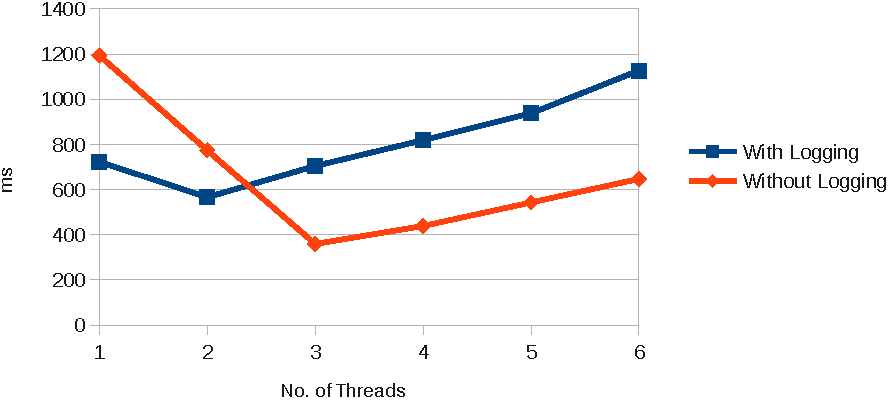
\includegraphics[width=\textwidth]{../experiment/latency-crop-split.pdf}
  \caption{Latency per request/client in nanoseconds}
  \label{fig:latency}
\end{figure}

\begin{figure}[ht]
  \centering
  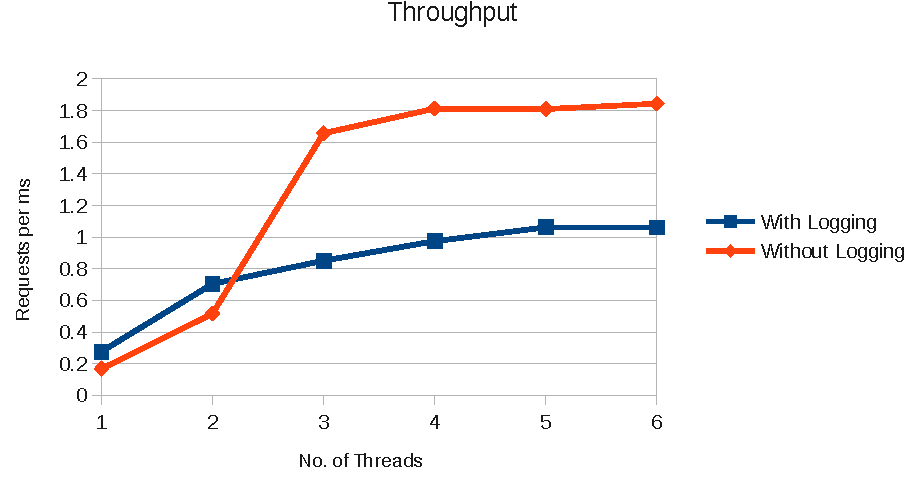
\includegraphics[width=\textwidth]{../experiment/throughput-crop-split.pdf}
  \caption{Throughput as requests per millisecond}
  \label{fig:throughput}  
\end{figure}

The experiment has been carried out using an increasing number of threads where each of them performed the same sequence of 9,000 update operations.

We can see that the latency drops for two threads (which I will use interchangably with 'client') and then slowly increases for each new thread that runs in parallel. The initial drop is expected since for few threads the experiment machine could actually simulate them in parallel (4 cores) which resulted in the samve overall running time but of course a smaller running time per thread. After that, computing limitations on the machine as well as logging overhead start to kick in giving measures of logging overhead from 74\% to 96\%.

These high values are also due to the fact that the clients and the server ran on the same machine, so there was no network traffic that could dominate the latency. Given the absolute values of fractions of milliseconds it is easy to see that any usage of an intermediate network would affect the latency measured and would definitely decrease the overhead percentage per request. However, given the pure character of the measurements (performed on the same machine without network delays and the only difference between the services being the disabled logging) we can assume that the reported percentage reflects the overhead induced by logging rather accurately.

Similarly, the throughput (requests per millisecond handled by the server) increases but soon reaches a plateau. By the same argument as before, the fact that the logging service can only process from 51\% to 58\% of the requests per millisecond compared to the service without logging illustrates the logging overhead very well.

We can conclude that, on the testing machine used, the overhead induced by logging approaches a constant of about 100\% in latency and a performance decrease of about 50\% in throughput. However, carrying out the experiment with multiple physical clients that do not suffer from being simulated on a limited-core machine as well as requesting the operations via a network would give a more realistic (and less artificial) testing environment.

Note that the architechture of my machine has a high impact on these numbers: 4 cores and a hard disk drive may not reflect the ideal environment. Multiple cores will allow for more realistic client simulation and a solid state disk would probably drastically reduce the overhead induced by logging as we have seen in the hardware comparison in the last assignment.

% -----
\subsection{Extensions}
\label{sec:pt5}
The group commit has been implemented in the logger which waits for a certain amount of log requests to be made before flushing them to disk once or alternatively flushing the queue of accumulated log requests after a certain time has passed since the last flush. The current implementation makes no exceptions for log requests from \texttt{init} for the sake of simplicity. This means that the first call to \texttt{init} blocks all other operations for the amount of time specified in the timeout property. After that the service greatly benefits from multiple clients accessing it in parallel because otherwise the logger would always have to time out before writing logs to disk, thus artificially decreasing the performance. Because of the toy example nature of our implementation, I have mostly tested the commits with \(K=1\) and a timeout of 0, thus practically disabling group commits. However, I have tested manually that operations block until the first init log entry has been written because of a timeout effect. Additionally I have checked that for sufficient parallel requests that exceed \(K\) the log is flushed accordingly.

% -----
% -----
% -----
\section{Implementation Notes}
\label{sec:notes}
In this section I want to briefly explain why I have made implementation decisions that might not have been intended by the assignment. I have chosen to not use the \texttt{unpin} method provided in the \texttt{MemoryMappedPinnable} because of multiple reasons. First it was not clear to me what I should use it for, especially with respect to the lacking documentation (both in the assignment text and the source code) such that I could only move on with my own interpretation.

Upon further thought I realized that you probably wanted us to implement some sort of the following procedure: make a log request, do not block immediately and pin the memory region, then block until the log is flushed to disk and unpin the region again because now the log is written and the data may be released to the underlying \texttt{MemoryMappedFile} buffers which may or may not write the data on disk. This would then be forced by the \texttt{Checkpointer}. However, given the late time of this realization as well as the necessary changes to the provided interfaces I decided to not implement these changes.

Instead I am blocking until the log has been flushed and only then write the pinned memory region. This could be harmful if we run the checkpointer only in very large intervals, thus cluttering the main memory of the machine because of never unpinning. However I consider this effect neglectable for the kind of toy experiments that we perform.

The fact of not unpinning memory has the effect that on update operations an overlap of \texttt{PinnedRegion}s would be detected. I circumvented this issue by removing the previous pinned region from the managing hash table which has the same effect as unpinning the region after insertion such that it is not occupied on update.

If we take into account that the implementation of this assignment was also possible only using internal memory I think that my implementation suits the purposes well, especially with  the checkpointer running in a rather frequent interval and my knowledge of the points that could be improved.

\end{document}
